%
% Descripción del modo de operación de BPS, presentación de cifrados que 
% preservan el formato.
% Proyecto Lovelace.
%

\subsection{Modo de operación}

%------------------------------------------------------------------------------
\begin{frame}{BPS}{Modo de operación}

  El modo de operación usado por \textit{BPS} es equivalente al modo de 
  operación CBC, ya que el bloque $BC_n$ utiliza el texto cifrado de la 
  salida del bloque $BC_{n-1}$, con la distinción de que en lugar de 
  aplicar operaciones \textit{xor} usa sumas modulares caracter por 
  caracter, y de que no utiliza un vector de inicialización.
  
\end{frame}

%------------------------------------------------------------------------------
\begin{frame}{BPS}{Modo de operación}

  \begin{figure}[H]
    \begin{center}
      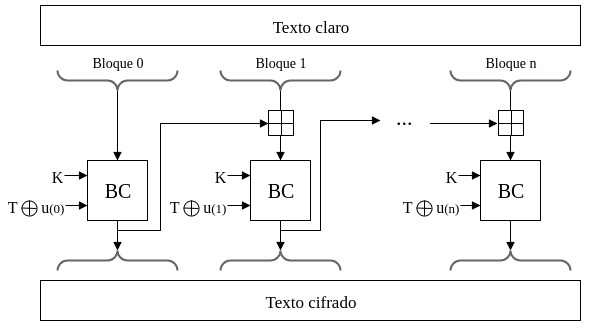
\includegraphics[width=1.00\linewidth]
      {../../../diagramas_comunes/bps/modo_de_operacion_bps}
      \caption{Modo de operación de \textit{BPS}.}
     \end{center}
  \end{figure}
  
\end{frame}

%------------------------------------------------------------------------------
\begin{frame}{BPS}{Modo de operación}

  Como se observó en la figura anterior, se utiliza un contador $u$ de 16 
  bits para aplicar una \textit{xor} al \textit{tweak} $T$ en la entrada de
  cada $BC$. 

  El \textit{xor} se aplica a los 16 bits más significativos de ambas mitades 
  de \textit{tweak}, debido a cada mitad de \textit{tweak} funciona de manera
  independiente en $BC$, y a que no se desea un traslape entre el contador
  externo e interno.
  
\end{frame}

%------------------------------------------------------------------------------
\begin{frame}{BPS}{Modo de operación}

  Con este modo de operación, cuando el texto en claro a cifrar no tenga 
  una longitud total que sea múltiplo de la longitud de bloque, el último 
  bloque recorre su cursor de inicio hasta que su longitud concuerde.
  
  \begin{figure}[H]
    \begin{center}
      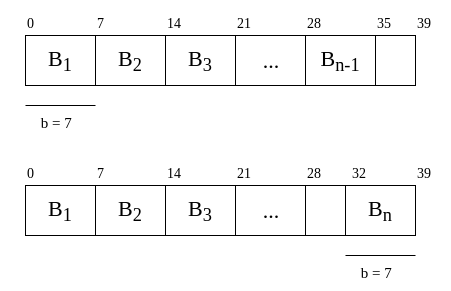
\includegraphics[width=0.5\linewidth]
      {../../../diagramas_comunes/bps/cursor_bps}
      \caption{Corrimiento de cursor de selección del ultimo bloque.}
     \end{center}
  \end{figure}
  
\end{frame}

%------------------------------------------------------------------------------
